% Template for PLoS
% Version 1.0 January 2009
%
% To compile to pdf, run:
% latex plos.template
% bibtex plos.template
% latex plos.template
% latex plos.template
% dvipdf plos.template

\documentclass[10pt]{article}

% amsmath package, useful for mathematical formulas
\usepackage{amsmath}
% amssymb package, useful for mathematical symbols
\usepackage{amssymb}

% graphicx package, useful for including eps and pdf graphics
% include graphics with the command \includegraphics
\usepackage{graphicx}
\usepackage{float} 

% cite package, to clean up citations in the main text. Do not remove.
\usepackage{cite}

\usepackage{color} 
\usepackage{multirow} 

% Use doublespacing - comment out for single spacing
%\usepackage{setspace} 
%\doublespacing


% Text layout
\topmargin 0.0cm
\oddsidemargin 0.5cm
\evensidemargin 0.5cm
\textwidth 16cm 
\textheight 21cm

% Bold the 'Figure #' in the caption and separate it with a period
% Captions will be left justified
\usepackage[labelfont=bf,labelsep=period,justification=raggedright]{caption}

% Use the PLoS provided bibtex style
\bibliographystyle{plos2009}

% Remove brackets from numbering in List of References
\makeatletter
\renewcommand{\@biblabel}[1]{\quad#1.}
\makeatother


% Leave date blank
\date{}

\pagestyle{myheadings}
%% ** EDIT HERE **


%% ** EDIT HERE **
%% PLEASE INCLUDE ALL MACROS BELOW

%% END MACROS SECTION

\begin{document}

% Title must be 150 characters or less
\begin{flushleft}
{\Large
\textbf{Effects of Beta and Delta/Theta Binaural Beats on Stroop Test}
}
% Insert Author names, affiliations and corresponding author email.
\\
Carles Tard\'io$^{1}$, 
Borja Sabio$^{1}$, 
Selin Akcakaya$^{1}$,
Xavier Duran$^{1}$,
Maria Blancas$^{1}$
\\
\bf{1} Interdisciplinary Master in Cognitive Systems and Interactive Media, Pompeu Fabra University, Barcelona, Spain

%$\ast$ E-mail: Corresponding author@institute.edu
\end{flushleft}

% Please keep the abstract between 250 and 300 words
\section*{Abstract}
Exposure to two tones of mildly different frequencies in each ear produces a phenomenon known as binaural auditory beats. Binaural beats are low-frequency pulsations in the amplitude and sound localization of a perceived sound. The resulting frequency of the binaural beat is the difference between the frequencies of both tones. Some reports suggest binaural beats can entrain EEG activity affecting states of consciousness, although few robust scientific studies have been published on the matter. In this study, the effects of binaural beats in beta and delta/theta range frequencies, associated with alertness and drowsiness states respectively, were examined through the Stroop test which has become over the years a reliable tool to measure reaction time and accuracy. The hypothesis of the study may be formulated as: “Exposure to binaural auditory beats in the EEG beta frequency ranges in comparison to delta/theta frequency ranges improves significantly performance in Stroop test”. In the experiment 20 healthy subjects were exposed to beta and delta/theta BB for 15min each sound. No statistically significant difference between the two conditions was found, neither in reaction time (\(F\)(1,19)=2.19, \(p\)\textgreater.1) [delta/theta (\(M\)=0.18, \(SD\)=0.15), beta (\(M\)=0.20, \(SD\)=0.17) ] nor in accuracy [\(F\)(1,19)=1.17, \(p\)\textgreater.1 ]. We suggest further studies could be performed extending the duration of the exposure to the binaural beats.

\section*{Introduction}
Binaural Beats are auditory brainstem responses which originate in the superior olivary nucleus of each hemisphere. They result from the interaction of 2 different auditory impulses, originating in opposite ears below 1000 Hz and which differ in frequency between 1 and 30 Hz \cite{oster1973auditory}. For example, if a pure tone of 400 Hz is presented to the right ear and a pure tone of 410 Hz is presented simultaneously to the left ear, an amplitude modulated standing wave of 10 Hz which is the difference between the two tones, is experienced as the 2 waveforms mesh in and out of phase within the superior olivary nuclei.
 
This binaural beat is not "heard" in the ordinary sense of the word (the human range of hearing is from 20-20,000 Hz). It is perceived as an auditory beat and theoretically can be used to entrain specific neural rhythms through the frequency-following response (FFR),the tendency for cortical potentials to entrain to or to resonate at the frequency of an external stimulus. \cite{smith1975far},\cite{wahbeh2007binaural},\cite{foster1990eeg}. The scientific term used for this synchronization process in the literature is "entrainment". Thus, it is theoretically possible to utilize a specific binaural-beat frequency as a consciousness management technique to entrain a specific cortical rhythm.
 
When the perceived beat frequency corresponds to the delta, theta, alpha, beta, or gamma range of brainwave frequencies, the brainwaves entrain to or move towards the beat frequency \cite{rogers1981methods}. As in the previous example, if a 400 Hz sine wave is played into the right ear and a 410 Hz one into the left ear, the brain is entrained towards the beat frequency 10 Hz, in the alpha range. Since alpha range is associated with relaxation, this has a relaxing effect. Beats in the theta range would have the effect of increasing alertness. An experiment with binaural sound stimulation using beat frequencies in the beta range on some participants and beat frequencies in  the delta/theta range on other participants found better vigilance performance and mood in those on the awake alert state of beta-range stimulation.\cite{owens1998binaural}, \cite{beatty1974operant}. Other studies exploring the effect of binaural beats on similar attention tasks have not been conclusive.\cite{wahbeh2007binaural},\cite{crespo2012effects}.
 
Since the discovery of binaural beats, the majority of studies on the matter come from environments related to the binaural beats industry and that actually make profit from them. There are, however, numerous self-reported cases of benefits on the matter. Considering the latter, an important factor that should not be dismissed as a possible explanation is the placebo effect.  With these considerations, there is a need for well-designed independent studies. As binaural beats are a cheap technology (there exist open source programs like Gnaural or Audacity to create them), any achievement in this area could be of public interest.\cite{crespo2012effects}

The aim of our research is to explore the effects of binaural beats on cognitive function, in particular in performing the Stroop test.

% You may title this section "Methods" or "Models". 
% "Models" is not a valid title for PLoS ONE authors. However, PLoS ONE
% authors may use "Analysis" 
\section*{Materials and Methods}
\subsection*{Experiment Design}
The experiment took place in a soundproof room at the facilities of Pompeu Fabra University. The equipment was composed by a pair of stereo headphones, a microphone and an iPad. The subjects were asked to wear the headphones during the whole experiment in order to block the noise from the exterior. The importance of not removing the headphones before the end of the experiment was specially remarked. Through the headphones, subjects were exposed to the specific binaural sounds mixed with pink noise as background, to make the binaural sounds imperceptible. Documentation of written consent and verbal and written explanations of the experiment were presented to the subjects before beginning the experiment. Participation posed no risk. 
 
The design of the experiment was “within subjects”, meaning that the same group of subjects was exposed to more than one condition. In this case, the conditions were the two binaural beats: the delta/theta and the beta one. The duration of the entire procedure was around 35 minutes. It consisted of two parts, each of them lasting around fifteen minutes, depending on the subject’s performance, with a break of five minutes in between. There were 21 participants, whose mean age was 28.1 years old, nine females and eleven males (one of them was removed from the data for taking off the headphones before the experiment finished). In both parts subjects had to perform the same tasks, having the two binaural beats as the main independent variable.
 
In order to keep subjects naïve to the purpose of the experiment, they were told it aimed at exploring color perception. The files that contained the sounds were renamed by a person external to the experiment so that they were double-blinded to the subjects as well as the conductors of the experiment. The latter was important in order to ensure that they did not influence participants by knowing which specific sound would be displayed in each part. The order of the sounds was counterbalanced through a randomized sound sequence where 10 random subjects were presented the beta binaural beats in the first part of the experiment and the delta/theta in the second one, and 10 other random subjects were presented the sounds in the reverse order. Each part of the experiment was divided again into two subparts:

1) The first subpart lasted nine minutes and consisted of a video displaying Ishihara color test plates. The Ishihara test consists in different plates with figures or patterns constituted of colored dots of diverging size that the subjects are asked to recognize among different colored dots that surround these figures or patterns.  \cite{rosenfield2009optometry}. The objective of the test is detecting color blindness.
 
In this part of the experiment, the subjects were presented with a set of images displaying numbers and shapes in colored backgrounds inserted on a video. The video was composed by seventeen number plates, six shapes plates and nine lines plates, each of them lasting for 15 seconds. For each one of them, they were requested to identify the number, line or shape they were able to see and report it through the microphone. The reason for conducting the Ishihara test was twofold: on the one hand it served to check whether any of the subjects was color-blinded (in which case he/she could not take the Stroop test of the second subpart of the experiment) and it also served to entertain subjects during the initial exposure to binaural beats, maintaining their focus without exhausting them. This was necessary because subjects needed to be exposed to the binaural beats for some minutes prior to undertaking the Stroop test.
 
2) The second subpart lasted around six minutes (depending on the subject’s performance) and it consisted of the Stroop test. Subjects had to perform the test using an iPad application they were shown before the experiment began. When the video with the Ishihara test had finalized, subjects had to start the Stroop test application themselves and proceed as they were instructed beforehand. Once this part was finished they had to remove the headphones and report to the examiners.
 
The Stroop test, based on the Stroop effect \cite{stroop1935studies}, measures cognitive flexibility, selective attention and psychomotor speed. It is considered a standard to assess interference in the reaction time of a task. For this experiment, we used the application "Encephalapp - Stroop Test" developed by Dr. Jasmohan Bajaj and freely available for iPad and other devices. This application has been used in prior studies of patients with liver disease as a predictive tool to assess minimal hepatic encephalopathy (MHE), which is often found in patients with cirrhosis and is difficult to diagnose \cite{Bajaj2013a}.
 
The nature of the presented stimuli during the test is the second independent variable of the experiment. First the subjects are presented a minimum of five rounds of ten neutral stimuli and then a minimum of five more rounds of ten incongruent stimuli. Any error made in any of the rounds makes the subject start the round again from the beginning, so the final number of rounds needed to complete 10 rounds will differ from one subject to another depending on the accuracy of the responses given.

In the phase of neutral stimuli (referred to in the application as Stroop-Off state) only colored symbols are presented on the screen and subjects are asked to tap the button corresponding to the name of the color of the symbol. In the incongruent phase (referred to in the application as Stroop-On state), colored names of colors are displayed on the screen, being the color of the word different to the color meant by it (e.g. the word RED written in green font). Subjects are then asked to tap the button corresponding to the color of the word (e.g. green), not the meaning of it (e.g. RED). The objective in both phases is to respond as quickly and accurate as possible. Any single reaction time is computed as well as the total number of rounds performed.

According to the developers of the application, OffTime (total time expended in neutral phase) can be interpreted in terms of psychomotor speed. In parallel with this, OnTime (total time expended in incongruent phase) refers to the psychomotor speed and cognitive flexibility. Therefore the interpretation of the total OffTime+OnTime value is composite of psychomotor speed and the interpretation of OnTime-OffTime is an isolated measure of cognitive flexibility.


\subsection*{Reaction time modeling}

Many studies on reaction time (RT) analysis identify that the preconditions for the analysis of variance and regression are not met\cite{Lachaud2011a}. First, RT distributions are usually positively skewed, with a long tail on the right of the mean, so that the assumption of normality is often false and the linear model cannot be applied without loss of data meaningfulness\cite{Whelan2010}. Inverse or logarithmic RT transformations can be applied to normalize the distribution\cite{Baayen2010}.

Second, single RT are not independent of each other and there exists a correlation between different trials in a sequence. The EncephalApp only considers sequences of 10 correct responses in a row to minimize this kind of dependencies, avoiding strategies to increase the speed of a response at the expense of accuracy\cite{Bajaj2013a}.

Third, fast guesses and distractions may influence significantly the measures of central tendency of the distribution. Outlier detection techniques are applied to remove unusual long latencies and physically impossible short RT, but not more than 5\% of all the correct responses. Sensitive filtering by outlier removal also normalizes the distribution\cite{Ratcliff1993}.

There exists other statistical strategies to analyse RT data different to an analysis of variance. Some try to find a better fit than the Gaussian normal for RT, like the ex-Gaussian, Gamma or Weibull distributions\cite{VanZandt2000}. Others, try to analyse the whole RT distribution and take advantage potential of repeated measures design instead of simplifying it to a measure of the central tendency of the aggregated data, like the Mixed Effects Model\cite{Baayen2008} or the Multilevel Modeling\cite{VanZandt2000}. The normalization of the distribution and the analysis of variance was used in this analysis for its robustness.

\subsection*{Data analysis}

The two within-subject factors analysed were the two levels of Stroop task (neutral, incongruent) and the two types of binaural beats frequencies (beta, delta/theta), making four different conditions. The dependent variables for the following statistical analyses were mean reaction times and accuracy. Accuracy was calculated as the number of errors per total correct targets.

The EncephalApp generated four data files for every subject, one per condition. The total of eighty files were merged and processed into two different files. The first one had all 4000 correct single item measurements, 50 per file; the other one, had the total time and the number of errors for each condition and subject. Only correct response times were taken into account.

The series of 50 reaction times were treated as independent variables each other, as the response to error latency and the fast guesses, the main sources for dependence, was eliminated on the experiment design by only considering sequences of 10 correct responses. Normality was tested for each distribution using the Shapiro-Wilk test of normality, but they didn't met the assumption as expected. Data transformations were applied to normalize the distributions. First of all, outliers beyond two times the standard deviation of the mean were removed independently for each subject, in each condition; then, a logarithmic transformation was applied to improve Gaussianity and the Shapiro-Wilk test was finally passed.

Data were collapsed over the responses to each subject and condition, and the mean was taken as a measure of central tendency. Reaction times to a single item and accuracy were subjected to a two-way repeated measures analysis of variance.

The data were analyzed with R, an open-source language and environment for statistical computing freely available at http://r-project.org. All data are reported as mean \(M\) $\pm$ standard deviation \(SD\).

% Results and Discussion can be combined.
\section*{Results}

The analysis yielded a main effect for the Stroop levels as expected, \(F\)(1,19)=16.94, \(p\)\textless.001, such that the log RT were significantly lower for the neutral (\(M\)=0.16, \(SD\)=0.14) than for the incongruent level (\(M\)=0.22, \(SD\)=0.17).

The average log RT for a single item in the Stroop test for the delta/theta frequency sound (\(M\)=0.18, \(SD\)=0.15) was slightly lower than for the beta frequency sound (\(M\)=0.20, \(SD\)=0.17), so the main effect of binaural beats frequencies were not significant, \(F\)(1,19)=2.19, \(p\)\textgreater.1. The interaction effect between the two factors was also not significant, \(F\)(1,19)=0.14, \(p\)\textgreater.1.

The errors on the Stroop task were reported to measure accuracy as the number of correct responses per total targets. An analysis of variance was performed to determine if the binaural beats frequencies had an effect on the accuracy for the Stroop task, but it was non significant, \(F\)(1,19)=1.17, \(p\)\textgreater.1.

\section*{Discussion}
In this paper, an experiment was performed in order to examine the effects of beta and delta/theta binaural beats and determine whether they have an impact on cognitive function, in particular in the performance on a Stroop test. No significant difference between the two conditions was found. The results yielded by this experiment provide no evidence to support the hypothesis proposed in the study: “Exposure to binaural auditory beats in the EEG beta frequency ranges in comparison to delta/theta frequency ranges improves significantly the performance in Stroop test”. However, a small effect was found in the opposite direction of the hypothesis, meaning delta/theta binaural beats were found to produce slightly better results regarding reaction time than beta binaural beats did. Although it was not the original purpose of the study, the difference between neutral and incongruent levels in Stroop test was also analyzed in order to confirm the observance of the Stroop effect. This effect was indeed assessed in a statistically significant lower reaction time for the neutral than for the incongruent level.

There is the possibility that 20 minutes duration was not sufficient to produce entrainment. Companies distributing commercial binaural beats usually claim that a long-term treatment (involving daily exposure to the sounds)  yields the desired effects. It may be that this lengthy treatment is necessary for the entrainment. Therefore, it could be interesting for further experiments to increase the exposure time to binaural beats to explore this possibility.

Addressing each of the two sessions in separate days could be a further improvement to the study, in order to minimize the possibility that any effect from the first part of the experiment remains in the second one. In the same way, more sessions could be arranged to increase the exposure to the sounds. On the other hand, these options would  decrease the controllability of the experiment.
 
A different approach would be performing the same experiment “between groups” instead of “within subjects”, meaning two groups of different people would be exposed to each of the sounds. This would avoid the possible learning curve implicit in performing the same task more than once. However, to avoid this inconvenience, in our experiment  the order of the sound was counterbalanced through a randomized sequence. In addition, the “between groups” approach presents some serious difficulties such as the need of a considerably big sample in order to avoid the natural variance present through subjects.



%\section*{References}
% The bibtex filename
\bibliographystyle{plos2009}
\bibliography{sample}

\section*{Figure Legends}

\begin{figure}[H]
\begin{center}
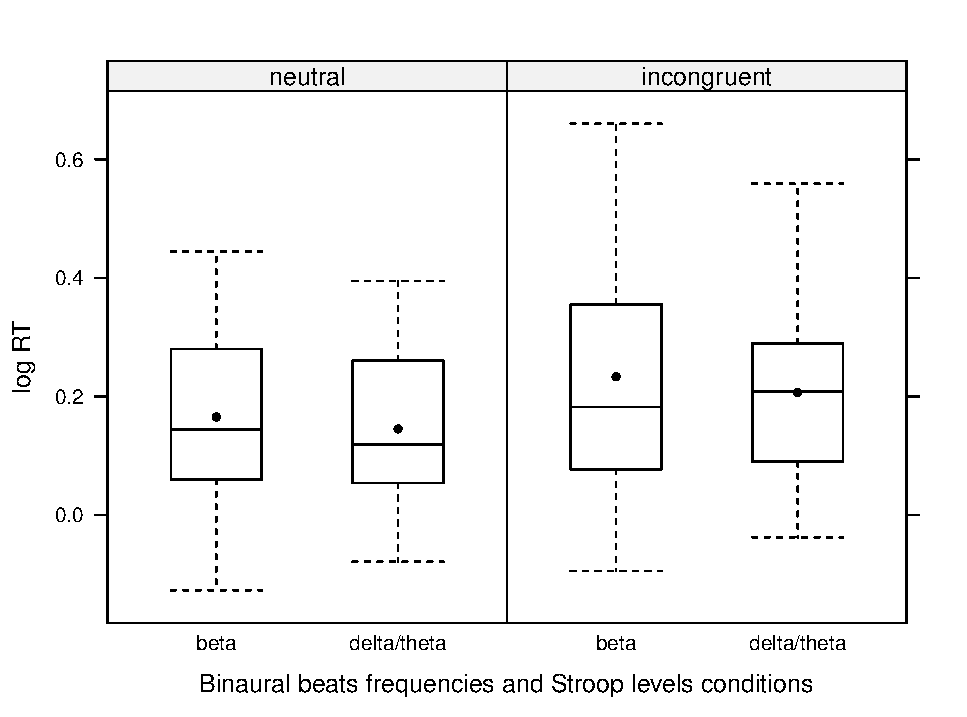
\includegraphics[width=4in]{logrt-eps-converted-to.pdf}
\end{center}
\caption{
{\bf Logarithm RT distributions for beta and deltha/theta frequencies.}
The dot in the middle of the plot stands for the mean log RT for each condition.
}
\label{figure_logrt}
\end{figure}

\begin{figure}[H]
\begin{center}
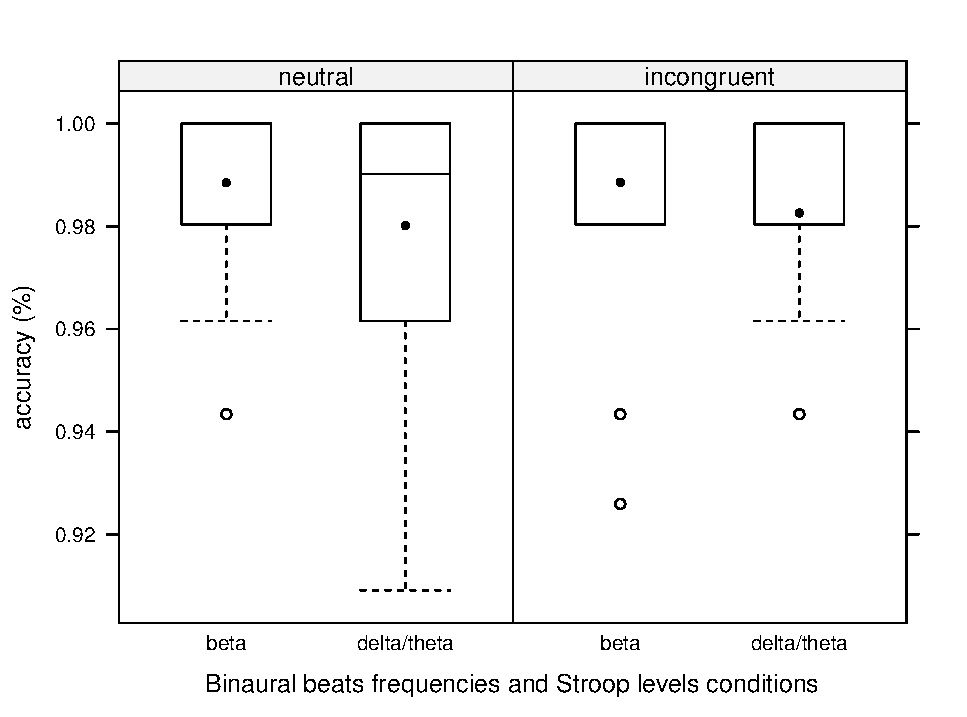
\includegraphics[width=4in]{accuracy-eps-converted-to.pdf}
\end{center}
\caption{
{\bf Accuracy distributions for beta and deltha/theta frequencies.}
The dot in the middle of the plot stands for the mean accuracy for each condition.
}
\label{figure_accuracy}
\end{figure}

\section*{Tables}

\begin{table}[!ht]
\caption{
{\bf Summary statistics for the four conditions and the dependent variables}
All data are reported as mean \(M\) $\pm$ standard deviation \(SD\).
}
\label{tab:summary}
    \begin{tabular}{|l|l|l|l|l|l|l|}
    \hline
    Stroop level & Beats frequency & RT & RT wo outliers & log RT & Total runs & Accuracy \\
    \hline
    \multirow{2}{*}{neutral} & beta & 1.25$\pm$0.20 & 1.21$\pm$0.19 & 0.16$\pm$0.15 & 5.60$\pm$0.94 & 0.99$\pm$0,02 \\
    & delta/theta & 1.23$\pm$0.20 & 1.19$\pm$0.17 & 0.14$\pm$0.14 & 6.05$\pm$1.40  & 0.99$\pm$0,03 \\
    \hline
    \multirow{2}{*}{incongruent} & beta & 1.36$\pm$0.31 & 1.31$\pm$0.28 & 0.23$\pm$0.19 & 5.60$\pm$1.09  & 0.99$\pm$0,02 \\
    & delta/theta & 1.33$\pm$0.24 & 1.27$\pm$0.21 & 0.21$\pm$0.15 & 5.90$\pm$0.85  & 0.99$\pm$0,02 \\
    \hline
    \end{tabular}
\end{table}



\end{document}

